\chapter{Basic operators}\label{Sec:SparcoOperators}

In this chapter we discuss the atomic operators that can be combined
to more complicated operators using the methods described in the
previous section.

\section{Elementary operators}\label{Sec:SparcoOpOnes}

The most elementary operators are created by the following commands:
\vspace*{.5em}

\noindent
\begin{tabular}{|p{2.4cm}p{9.4cm}|}
\hline
\mlcmd{opEye(m,n)}
& Creates an $m\times n$ operator with ones on the diagonal. When
  omitted, $n$ is set to $m$. Calling \mlcmd{opEye} without arguments
  creates an operator representing the scalar 1.\\
%
\mlcmd{opDirac(n)}
& Same as \mlcmd{opEye(n,n)}. When omitted, $n$ is set to 1. \\ 
%
\mlcmd{opZeros(m,n)}
& This creates an identically zero $m\times n$ operator. When omitted,
  $n$ is set to $m$. Calling \mlcmd{opZeros} without arguments creates
  an operator representing the scalar 0.\\
\mlcmd{opOnes(m,n)}
& This creates an $m\times n$ operator consisting of all ones. When
  omitted, $n$ is set to $m$. Calling \mlcmd{opOnes} without
  arguments creates an operator representing the scalar 1. \\
\mlcmd{opDiag(d)}
&  Creates an operator corresponding to the diagonal matrix with
   elements $d$. \\ 
\mlcmd{opWindow}
& Creates a diagonal operator for multiplication by one of the window
function given in Appendix \ref{Sec:SparcoWindowFunc}. \\
\hline
\end{tabular}

\section{Wrappers}\label{Sec:SparcoOpMatrix}

To allow existing operators in the form of classes, functions, or
matrices to be used in combination with \spot{}, a number of wrapper
functions are provided.
\vspace*{.5em}

\noindent
\begin{longtable}{|p{2.4cm}p{9.4cm}|}
\hline
\mlcmd{opMatrix(A)}
& Generates a wrapper operator for $A$. When $A$ is a class it must
  implement the \mlcmd{mtimes}, \mlcmd{ctranspose}, \mlcmd{size}, and
  \mlcmd{isreal} methods. A description of the underlying operator
  used when displaying the operator can be passed as an additional
  parameter. \\
\mlcmd{opFunction}
& Generates a wrapper operator for a function. For calling details
  type \mlcmd{help opFunction}. This function can also be used as a
  prototype for new wrapper functions supporting different
  function interfaces. \\
\mlcmd{opClass}
& Generates a wrapper operator for a class object. The only
  requirement on the object is that implements the \mlcmd{mtimes} and
  \mlcmd{ctranspose} methods. Type \mlcmd{help opClass} for calling
  details. \\
\hline
\end{longtable}

\section{Fast transformations}\label{Sec:SparcoOpFFT}

Operators for a number of standard fast transformations such as the
discrete cosine and Fourier transform are provided:

\begin{longtable}{|p{3.1cm}p{8.7cm}|}
\hline
\mlcmd{opDCT(m,n)}
& Creates a one-dimensional ($n=1$) or two-dimensional discrete cosine
  transform operator for vectorized $m\times n$ matrices. \\ 
\mlcmd{opFFT(m,n)}
& Creates a one-dimensional ($n=1$) or two-dimensional discrete
  Fourier transform operator for vectorized $m\times n$ matrices. The
  argument for $n$ is optional for one-dimensional transforms. An
  optional extra boolean flag can given to obtain a DFT where the
  zero-frequency component is centered. \\
\mlcmd{opHaar(m,n,l)}
& Creates a one-dimensional ($n=1$) or two-dimensional Haar wavelet
  transform with $l$ levels (by default 5 levels are used). Both $m$
  and $n$ must be powers of 2. This operator is a wrapper to the
  \mlcmd{opWavelet} operator. \\
\mlcmd{opHadamard(n)}
& Creates a operator representing a symmetric Hadamard matrix of order
  $n$. The underlying Hadamard matrix is constructed by repeatedly
  applying Sylvester's construction, starting with scalar 1. As a
  result, $n$ has to be a power of 2. Due to the inherent structure,
  multiplication can be done efficiently without constructing the
  matrix explicitly. \\
\mlcmd{opHeaviside(n)}
& Creates an operator representing the $n\times n$ Heaviside basis
  which consists of zero entries above the diagonal and ones on and
  below the diagonal. \\
\mlcmd{opToeplitz(m,n,v)}
& This function can be used to create operators for both Toeplitz and
  circular matrices of size $m\times n$, generated based on a given
  vector $v$ of entries. The type and optional column normalization is
  specified using additional parameters. For Toeplitz matrices $v$
  needs to contain $m+n-1$ entries. The first $m$ represent the first
  row while the last $n-1$ entries appear on the top row from the
  last to the second column. For circular matrices $v$ has length
  $k := \max(m,n)$ and represent the entries of the first column of
  the $k\times k$ circular matrix. Multiplication is implemented using
  the fast Fourier transform. \\
\mlcmd{opToepGauss(m,n)}
& Shortcut for \mlcmd{opToeplitz} with Gaussian $v$. \\
\mlcmd{opToepSign(m,n)}
& Shortcut for \mlcmd{opToeplitz} with random sign $v$. \\
\mlcmd{opWavelet}
& Wrapper for the discrete wavelet transformation implemented in the
  Rice wavelet toolbox \cite{RWT}. Type \mlcmd{help opWavelet} for
  details.\\
\hline
\end{longtable}

\noindent The following two fast transformation operators require
external software that could not be included in the distribution of
\spot{}. For those operators to work, the underlying implementation
has to be installed separately first.

\noindent
\begin{longtable}{|p{2.4cm}p{9.4cm}|}
\hline
\mlcmd{opCurvelet}
& This routine provides an interface to the discrete curvelet
transformation \cite{CandDemaDonoYing:2005} implemented in CurveLab
2.0 \cite{Curvelet}. \\
\mlcmd{opSurfacelet}
& This routine provides an interface to the discrete surfacelet
transformation \cite{LuDo:2007} implemented in the Surfacelet Toolbox
\cite{SurfaceletToolbox}. \\
\hline
\end{longtable}

\section{Random ensembles}

Spot provides a number of operator for random ensembles:

\begin{longtable}{|p{2.5cm}p{9.3cm}|}
\hline
\mlcmd{opBinary}
& Creates and operator for a matrix with i.i.d.\@ binary 0/1
entries. This function provides two modes of operation: one in which
the underlying matrix is explicitly formed and one which in which the
columns are generated as needed. The latter mode allows for the
construction of large operators whose matrices would not fit in
memory.\\
\mlcmd{opGaussian}
& Generates a Gaussian ensemble, i.e., an operator with randomly
generated normally distributed entries. There are a number of modes to
specify between an explicit or implicit underlying matrix and whether
the columns should be scaled to one. One additional mode for explicit
matrices allows the construction of ensembles with orthonormal rows.\\
\mlcmd{opBernoulli}
& Similar to \mlcmd{opBinary} but with random $\pm 1$ entries. It has
two additional modes that scale all columns to have unit Euclidean
norm.\\
\mlcmd{opSparseBinary} \mlcmd{(m,n,d)}
& This function creates an $m\times n$ sparse binary ensemble in which
each column contains $\min(m,d)$ ones at random locations. The default
number of non-zero entries in each column is set to $d=8$.\\
\hline
\end{longtable}

\section{Convolution}
One and two-dimensional convolution operators can be constructed using
the \mlcmd{opConvolve} function:
\begin{codeblock}
opConvolve(m,n,kernel,offset,mode)
\end{codeblock}
The first two parameters $m$, and $n$ indicate the size of the
vector/matrix $f$ upon which the convolution is applied. The next
parameter gives the convolution kernel and is followed by the offset
and mode parameters.  The offset indicates where the center of the
convolution kernel lies, and is set to \mlcmd{[1,1]} by default.
There are three possible modes, illustrated on one-dimensional vectors
in Figure \ref{Fig:SparcoConvolution}: regular, truncated, and
cyclic. In the regular mode we convolve $f$ with the kernel around its
offset. Let $g$ denote the kernel and assuming both $f$, and $g$ are
column vectors of length $m$, and $n$ respectively. Then the resulting
vector $f*g$ is of length $m+n-1$, unless the offset is less than one
or exceeds $n$. In the latter case, the kernel is pre or post padded
with zeros prior to convolution. When using truncated or cyclic
convolution the size of the resulting matrix or vector matches that of
$f$. The truncated mode performs regular convolution followed by a
cropping operation to obtain only the influences on the existing
domain (compare values within dotted line in Figure
\ref{Fig:SparcoConvolution}(c,d) with plots (e,f)). In the cyclic
mode, everything that falls outside the domain is wrapped back to the
other end. All modes are implemented using the discrete Fourier
transformation.

\begin{figure}
\begin{tabular}{cc}
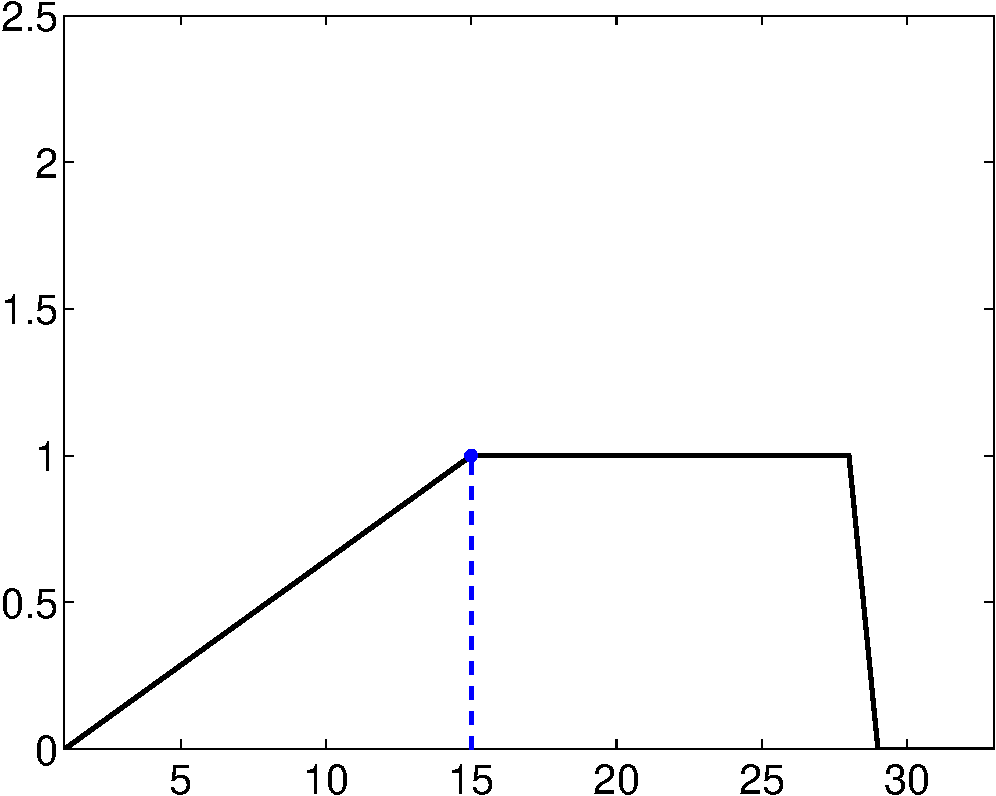
\includegraphics[width=0.425\textwidth]{./FigSparcoConvMask} &
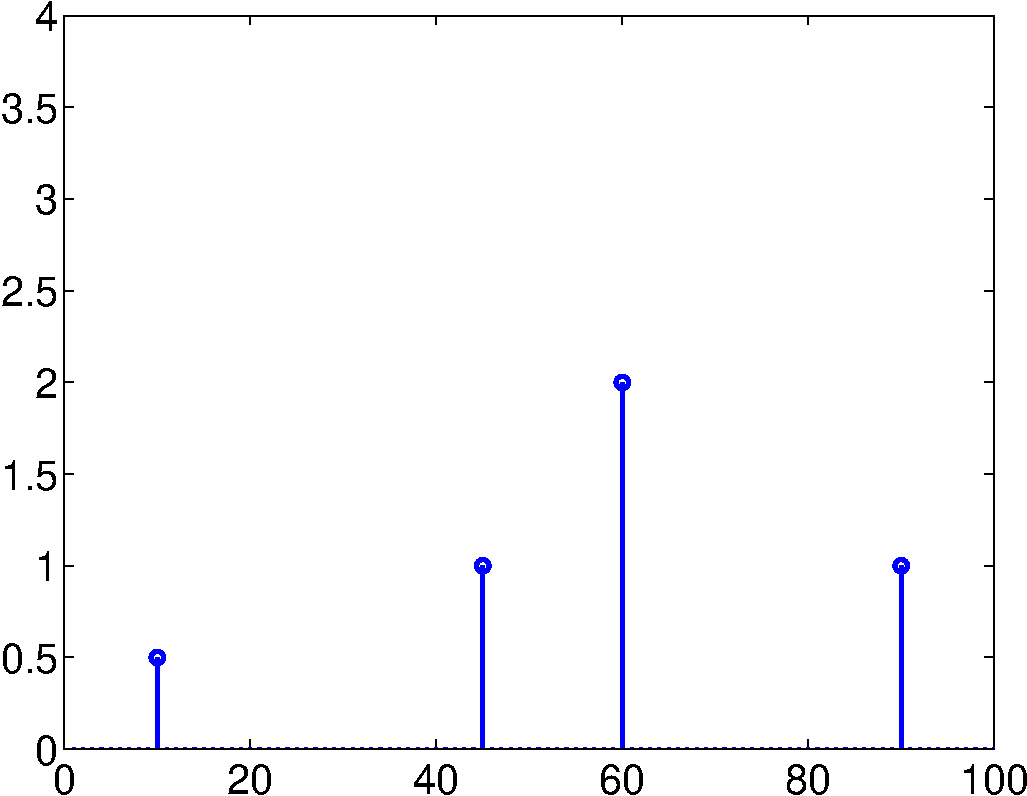
\includegraphics[width=0.425\textwidth]{./FigSparcoConvFun} \\
({\bf{a}}) & ({\bf{b}}) \\
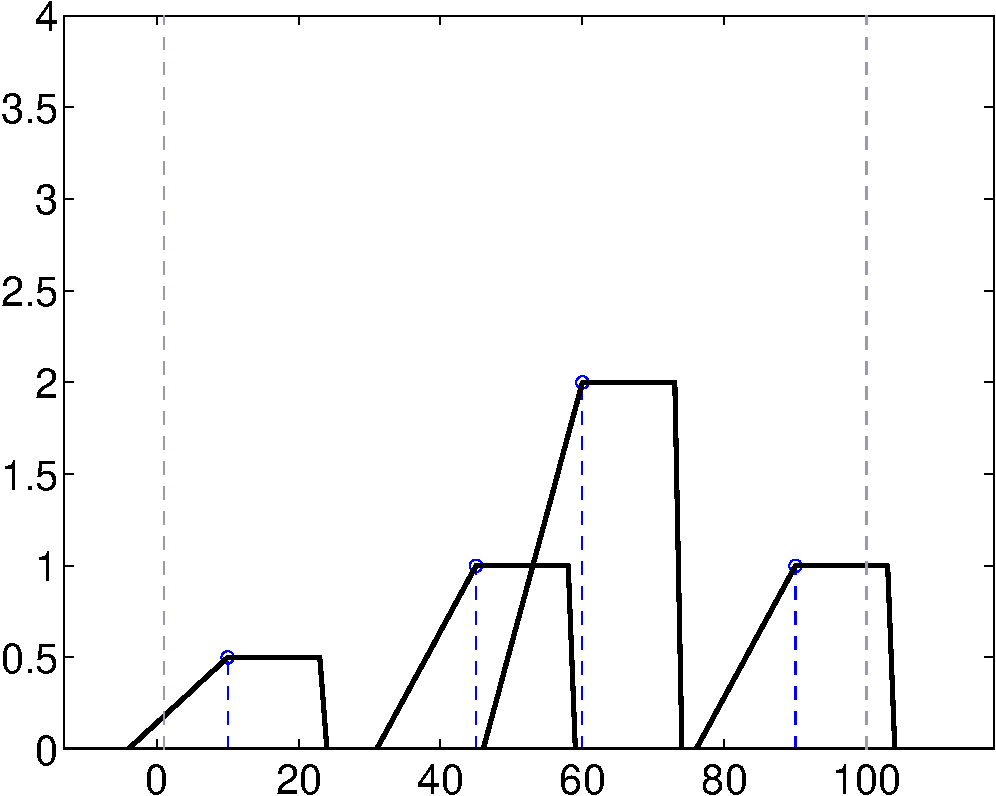
\includegraphics[width=0.425\textwidth]{./FigSparcoConvRegular1} &
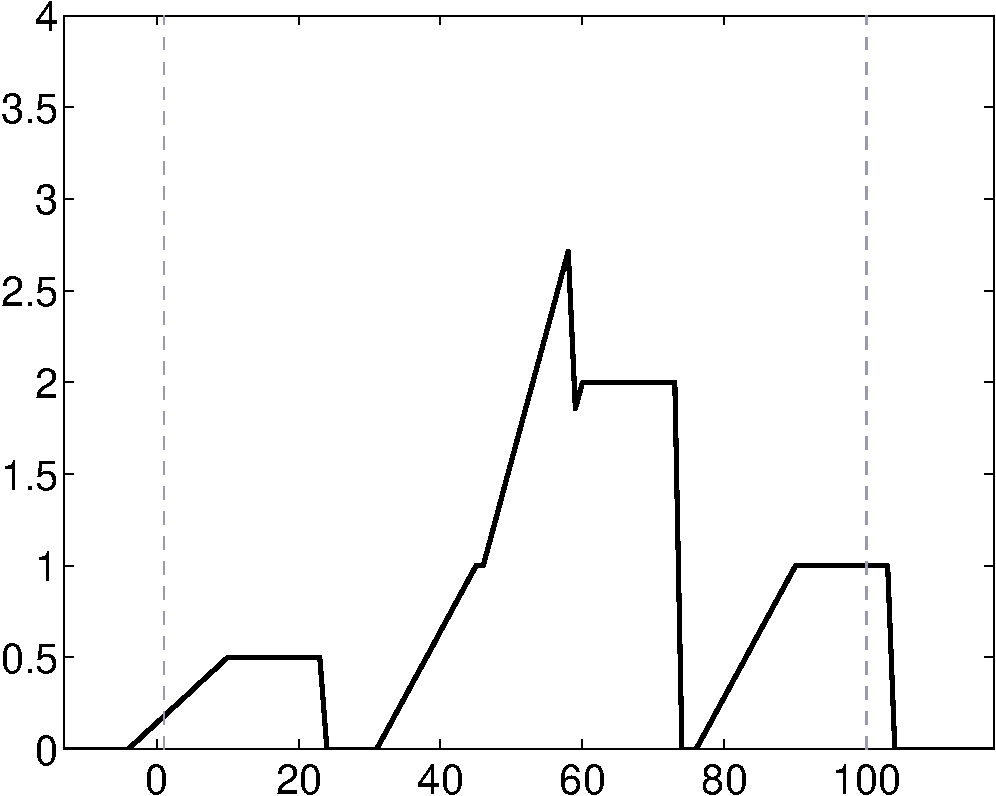
\includegraphics[width=0.425\textwidth]{./FigSparcoConvRegular2} \\
({\bf{c}}) & ({\bf{d}}) \\
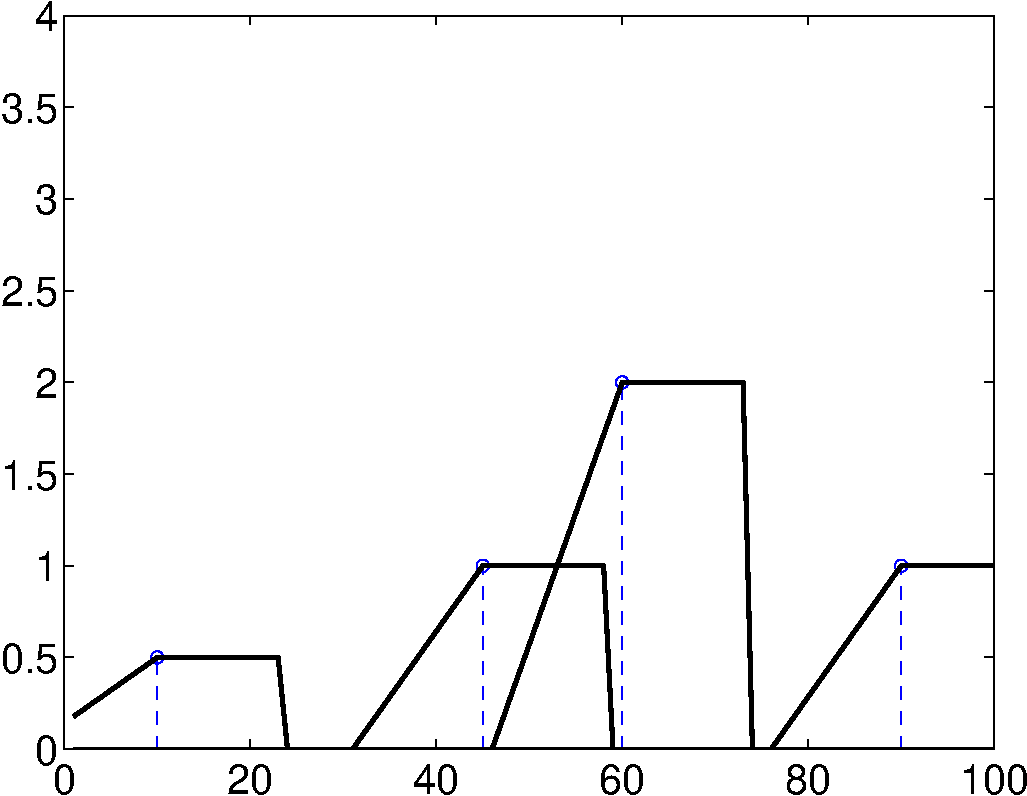
\includegraphics[width=0.425\textwidth]{./FigSparcoConvTrunc1} &
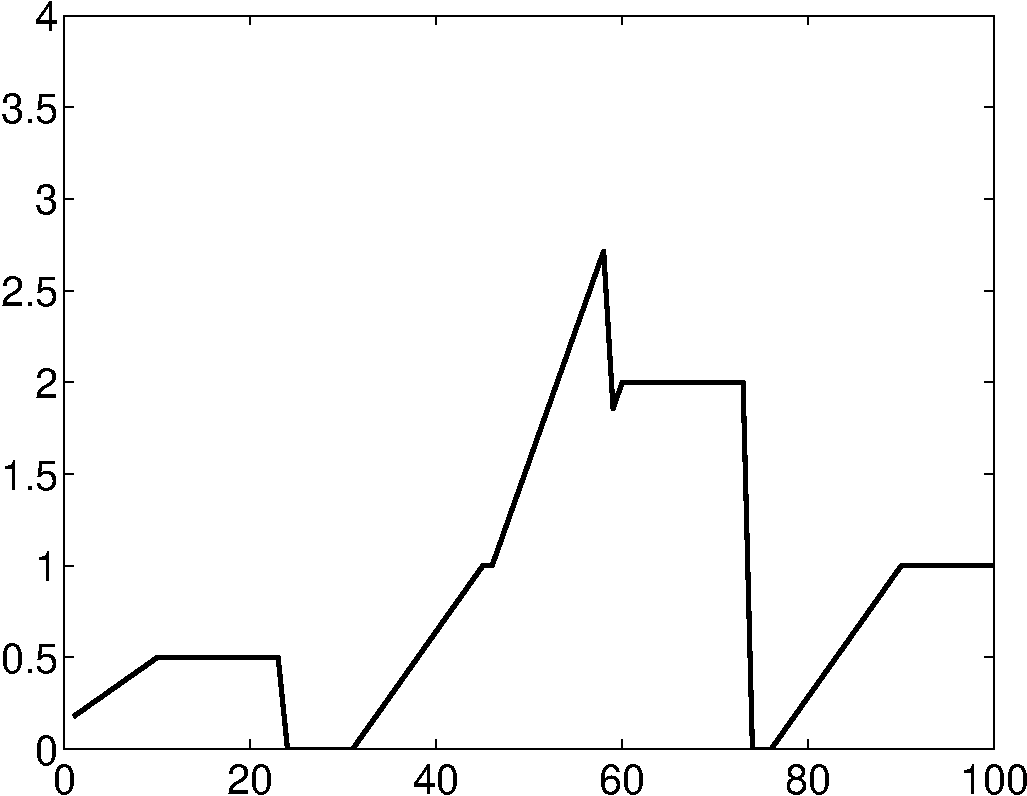
\includegraphics[width=0.425\textwidth]{./FigSparcoConvTrunc2} \\
({\bf{e}}) & ({\bf{f}}) \\
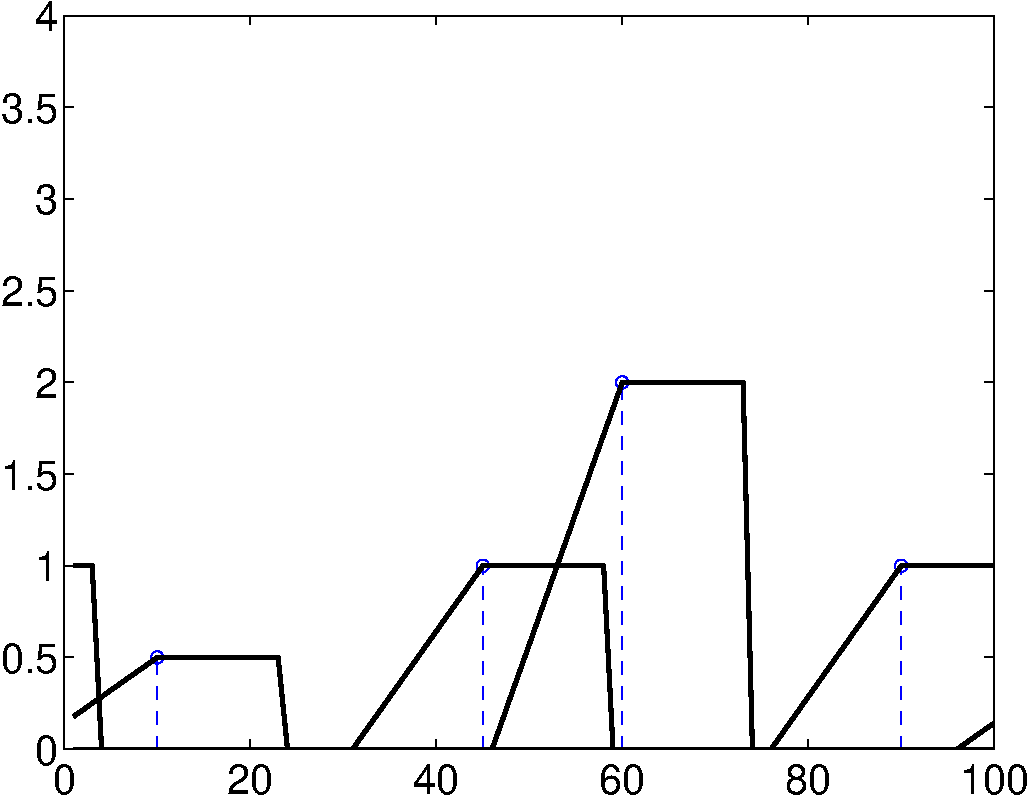
\includegraphics[width=0.425\textwidth]{./FigSparcoConvCycl1} &
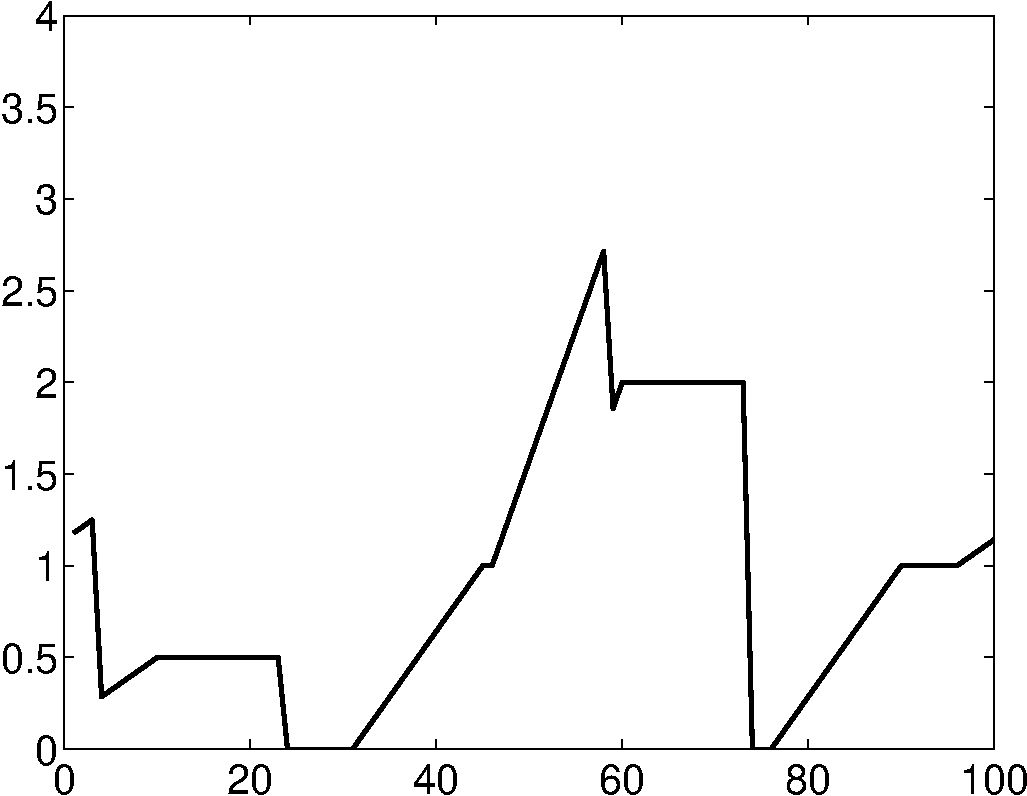
\includegraphics[width=0.425\textwidth]{./FigSparcoConvCycl2} \\
({\bf{g}}) & ({\bf{h}})
\end{tabular}
\caption{Illustration of the one-dimensional convolution operator; (a)
  convolution mask, (b) function, (c--d) regular convolution before
  and after summation, (e--f) truncated convolution, and (g--f) cyclic
  convolution.}\label{Fig:SparcoConvolution}
\end{figure}

%%% Local Variables: 
%%% mode: latex
%%% TeX-master: "manual"
%%% End: 
